\documentclass[12pt]{article}

\usepackage{amsmath}
\usepackage[authoryear,round]{natbib}
%\usepackage{hyperref}

\textwidth=6.2in
\textheight=8.5in
\oddsidemargin=.1in
\evensidemargin=.1in
\headheight=-.3in

\newcommand{\scscst}{\scriptscriptstyle}
\newcommand{\scst}{\scriptstyle}
\newcommand{\Rfunction}[1]{{\texttt{#1()}}}
\newcommand{\Rmethod}[1]{{\texttt{#1}}}  
\newcommand{\Rclass}[1]{{\texttt{#1}}}
\newcommand{\Robject}[1]{{\texttt{#1}}}
\newcommand{\Rpackage}[1]{{\textit{#1}}}
\newcommand{\code}[1]{{\texttt{#1}}}
\bibliographystyle{plainnat}
\def\tm{$^{\rm \text{TM }}$}

\title{Analysis of High Throughput Flow Cytometry Data using
\Rpackage{plateCore}}

%%%%%%%%%%%%%%%%%%%%%%%%%%%%%%%%%%%%%%%%%%%%%%%%%%%%%%%%%%%%%%%%%%%%%%%%%%%
\usepackage{Sweave}
\begin{document}
\maketitle

\clearpage
%%%%%%%%%%%%%%%%%%%%%%%%%%%%%%%%%%%%%%%%%%%%%%%%%%%%%%%%%%%%%%%%%%%%%%%%%%%%%%
\section*{Abstract}
\subsection*{Background}
Flow cytometry (FCM) software packages from R/Bioconductor, such as flowCore
and flowViz, serve as an open platform for development of new analysis tools and
methods. We created a new package, \Rpackage{plateCore}, that extends the
functionality in these core packages to enable automated isotype-based gating
and make the processing and analysis of plate-based data sets from
high throughput FCM screening experiments easier.

\subsection*{Methods}
\Rpackage{plateCore} was used to analyze the data from a BD FACS CAP screening
experiment where 5 Peripheral Blood Mononucleocyte Cell (PBMC) samples  were
assayed for 189 different human cell surface markers. This same dataset was
also manually analyzed by a cytometry expert using the FlowJo data analysis
software package (TreeStar, Ashland OR).

\subsection*{Results}
Positive markers identified using \Rpackage{plateCore} are in good agreement
with those found using manual analysis.

\subsection*{Conclusions}
\Rpackage{plateCore} provides a reproducible, objective platform for analyzing
high throughput FCM experiments. The R/Bioconductor implementation allows
bioinformaticians and statisticians access to the data, which should further
the development of automated analysis methods.

\clearpage
%%%%%%%%%%%%%%%%%%%%%%%%%%%%%%%%%%%%%%%%%%%%%%%%%%%%%%%%%%%%%%%%%%%%%%%%%%%%%%%
\section*{Introduction}

While there are a number of different software packages available for analysis
of FCM data, these programs are often ill-suited to the development of new
methods needed for analyzing high-throughput FCM studies. Flow Cytometry High
Content Screening (FC-HCS) experiments generate large volumes of data, and a
systematic approach to preprocessing, gating (i.e. filtering), and summarizing
results is needed for robust analyses. Automation of these steps would allow
analysis pipelines to be robust, objective, and match the high-throughput
capacity of modern cytometers. Unfortunately, current approaches to FC-HCS
analysis are semi-automated at best, and they often require significant
subjective and error-prone manual intervention to identify cells of interest
\citep{Maecker2005}. It is therefore desirable to develop programmatic
approaches to process FCM data.

FCM packages available through the Bioconductor \citep{BIOC} project provide an
open platform that can be used by cytometrists, bioinformaticians, and
statisticians to collaboratively develop new methods for automated FC-HCS
analysis. The basic data processing tools for importing, transforming, gating,
and organizing raw FCM data are in the \Rpackage{flowCore} package
\citep{hahne2009}, and the visualization functions are in \Rpackage{flowViz}
\citep{sarkar2008ufv}. The Bioconductor model for FCM data analysis facilitates
the development of new analysis methods, since the overhead associated with
accessing and visualizing FCM data is handled by \Rpackage{flowCore} and
\Rpackage{flowViz}. The availability of \Rpackage{flowCore} and
\Rpackage{flowViz} has enabled the creation of new tools for quality assessment
of large FCM experiments, such as \Rpackage{flowQ} \citep{lemeurFQ}, and
model-based clustering and automated gating, such as \Rpackage{flowClust}
\citep{lo2008}.

We have developed an R package (\Rpackage{plateCore}) that also takes advantage
of the functionality in \Rpackage{flowCore} and \Rpackage{flowViz} to create
methods and data structures for processing large, plate-based FCM datasets.
Additionally, we have implemented new tools to make it easier to integrate
textual descriptions of plate layouts and also functions for automated gating
based on non-parametric analysis of negative control wells. This study presents
results from an automated \Rpackage{plateCore} analysis of a PBMC lymphocyte
FACS CAP data set, which included 189 different antibody-dye conjugates
and their controls arranged on a 96-well plate. The \Rpackage{plateCore} output
was compared to an analysis by an expert cytometrist using FlowJo to evaluate
the performance of the automated approach.

\Rpackage{plateCore} is not designed to be a GUI driven end-user tool, but
rather to help develop a standardized platform for the analysis of FC-HCS data.
These analyses often represent a collaborative effort between cytometry experts
who generate the data and the quantitative individuals who help deal with the
large volume information. In order for this collaboration to work, the
cytometrists must have confidence in the results of the automated analysis. To
this point, we demonstrate the equality of our results to those produced by an
expert cytometrist using FlowJo.

%%%%%%%%%%%%%%%%%%%%%%%%%%%%%%%%%%%%%%%%%%%%%%%%%%%%%%%%%%%%%%%%%%%%%%%%%%%%%%%%
\clearpage
\section*{Materials and Methods}
\subsection*{Flow Cytometry Data}

The data analyzed in this study was part of the initial set of experiments
used to validate the BD FACS CAP platform. BD FACS CAP was designed as a cell
characterization tool to screen for the presence of a large number of different
human cell surface markers, and it was important to show that the assay was
able to correctly identify positive and negatively staining markers on a well
studied cell population, such as PBMC lymphocytes. Previously
frozen PBMC samples from two donors were analyzed on a BD FACS Calibur using BD
FACS CAP staining plates. The analysis was performed on 96-well plates with 189
different antibodies arrayed three per well in 63 test wells, along with 30
isotype control wells and three unstained controls. The complete list of BD
FACS CAP antibodies can be found at
http://www.bd.com/technologies/discovery\_platform/BD\_FACS\_CAP.asp. FCM files
for the 5 plates (two for Donor 1 and three for Donor 2), are available for
download from http://www.ficcs.org.

%%%%%%%%%%%%%%%%%%%%%%%%%%%%%%%%%%%%%%%%%%%%%%%%%%%%%%%%%%%%%%%%%%%%%%%%%%%%%%%%
\subsection*{\Rpackage{plateCore}}

The \Rpackage{plateCore}
scripts used to perform the analysis are provided in supplementary materials.
Briefly, the FCM files were first processed using a combination of static
gates(\Robject{rectangleGate}) and data driven gates (using
\Robject{norm2filter} and \Rpackage{flowCore}) to pick out the lymphocytes in
the forward (FSC) and side scatter (SSC) channels.  The
quality of the data was then assessed by looking for fluidic events such as
bubbles, pressure drops, or large aggregates that can shift the baseline
fluorescence readings. Fluidic events can often be identified by plotting the
empirical cumulative density (ecdf) plots of FSC values for each well, and
looking for distributions shifted relative to other wells \citep{lemeur2007}.
Based on the ecdf plots, several wells were further investigated by cytometry
experts who determined that the shifts were in an acceptable range. Next the
threshold between positive and negative cells were determined using the isoytpe
controls, which provided a gross estimate of non-specific binding in the
primary antibodies. One-dimensional gates were created using using the isotype
thresholds, and these gates were applied to identify cells that are positively
stained for each marker.

An example of the progression from raw FCM data files to a completed
\Rpackage{plateCore} analysis is shown in Figure~\ref{fig:analysis}. List mode
FCS files for a single plate were read into a \Robject{flowSet} using
\Rpackage{flowCore}, and then a \Robject{flowPlate} was created by integrating
the plate annotation file with the \Robject{flowSet}. The \Robject{flowPlate}
was then compensated, data quality was assessed, and gates were set according
to a negative control. These control gates were then applied to test wells to
find cells that had specific staining in channels of interest.

\begin{figure}
\centering
\includegraphics[width=7in,height=6in]{analysisSteps.pdf}
\caption{Typical FC-HCS plate workflow on the left and corresponding steps from
a PBMC lymphocyte \Rpackage{plateCore} analysis on the right. Compared to
analyses performed using existing GUI FCM tools, \Rpackage{plateCore} can
reduce the level of subjectivity associated with creating the negative control
gates and also makes it easier to aggregate multiple plates into an experiment
level object for visualization and reporting. Providing \Rpackage{plateCore}
scripts along with the raw FCM data for FC-HCS experiments helps to ensure that
analysis is transparent and reproducible.}
\label{fig:analysis}
\end{figure}

%%%%%%%%%%%%%%%%%%%%%%%%%%%%%%%%%%%%%%%%%%%%%%%%%%%%%%%%%%%%%%%%%%%%%%%%%%%%%%%
\subsection*{FlowJo}

In addition to \Rpackage{plateCore}, the five PBMC plates were also analyzed
using FlowJo. First, an analysis template was created where test wells and
their corresponding isotype control well were assigned to one of 30 groups.
Wells in each group had similar sets of antibody-dye conjugates, and
the expression threshold (\emph{i.e.}, isotype gate) was initially set using
the isotype control well. Data for each plate was imported into FlowJo using
the template and lymphocytes were selected using a morphology (FSC-SSC) gate.
Event data for the isotype well was then visualized on a log scale, and the
expression threshold for each stained channel was set by picking a value that
lies above the bulk of the events. For BD FACS CAP, the isotype gates were
initially set so that approximately 1\% or less of the events in the isotype
well were above the threshold. These gates were then applied to the test wells,
and the gates were moved up or down depending upon positive and negative test
well populations. If the the population of cells in positive wells was much
higher than the isotype gate, then the gate was moved up to help reduce false
positives associated with non-specific staining.  Similarly, if the isotype
gate was higher than negative samples, the gate would be moved down to ensure
that positive cells were classified correctly. The percentage of cells above
the threshold for each of the 189 antibodies was then exported for each plate.

%%%%%%%%%%%%%%%%%%%%%%%%%%%%%%%%%%%%%%%%%%%%%%%%%%%%%%%%%%%%%%%%%%%%%%%%%%%%%%%
\section*{Results}

Although this study focuses on comparing two different FC-HCS analysis methods,
it is important to consider the orignal goal of the experiment used to generate
the data when interpreting the results. BD FACS CAP was designed to provide a
standard assay platform for screening a large number of markers on many
different cell types. The validation effort for BD FACS CAP included running
the assay on well-charaterized cell types to find markers with either positive
or negative staining, and comparing these results to published cell expression
profiles in the literature. The PBMC lymphocyte staining results presented in
the following section represent one of the cell types used for validating the
technology.


%%%%%%%%%%%%%%%%%%%%%%%%%%%%%%%%%%%%%%%%%%%%%%%%%%%%%%%%%%%%%%%%%%%%%%%%%%%%%%%
\subsection*{FlowJo Output}

Descriptions of marker expression profiles for particular cell populations in
flow cytometry often use terms like positive-negative, or bright-dim, to
qualify the amount of target present. Since FACS CAP is a
standard platoform for screening a wide range of cell types, and antibody
concentrations were not optimized for these PMBC samples, results are reported as
the percentage of cells above the isotype gate rather than positive or
negative. Follow-up studies, including single color titrations and competition
experiments, are needed to definitively say whether a marker is present.
These additional analyses of markers that have been characterized
using FACS CAP show that markers with $\ge$ 90\% of the cells above the isotype
threshold are usually confirmed as positive, while staining in markers with
$\le$ 10\% of cells above the isotype threshold is often the result of
non-specific binding (data not shown). Note that these percentages refer to the
fraction of cells above the isotype threshold, but this does not necessarily
imply heterogeneous staining in multiple populations.

Automating the creation and modification of isotype gates made by cytometrists
analyzing BD FACS CAP data using FlowJo is challenging. Cytometrists adjust
gates based on expert knowledge about the performance of specific antibody
types and dyes, or after identifying positive or negative test samples. If the
isotype gate cut off the bottom portion of a positive cell population in a test
well, then the gate was moved down.  Similarly, if the the isotype gate
included too many cells from negative test wells, it was moved up. Results from
the FlowJo based gating of replicate PBMC plates are shown in
Figure~\ref{fig:replicate}. Detailed results for each marker are not
presented in this study, but since the majority of antibodies on the FACS
CAP staining plate are known to bind different leukocytes, it is not surprising
that a large fraction would be identified as positive on PBMCs. Markers such as
CD44, CD45, CD47, and CD59 are broadly expressed on lymphocytes and were
positive (>99\%) in this study.

%%%%%%%%%%%%%%%%%%%%%%%%%%%%%%%%%%%%%%%%%%%%%%%%%%%%%%%%%%%%%%%%%%%%%%%%%%%%%%
\subsection*{\Rpackage{plateCore} versus FlowJo}
The automated approach to gating in \Rpackage{plateCore} determines the
threshold using isotype control wells. The gate (G$_{ij}$) for isotype $i$,
channel $j$ is set according to:
\begin{equation}
\text{G}_{ij} = \text{MFI}_{ij} + 4 \text{MAD}_{ij},
\label{isoGate}
\end{equation}
where MFI is the Median Fluoresence Intensity and MAD is Median Absolute
Deviations on a linear scale. The choice of 4 MADS is an attempt to set the
gate above the 99th percentile of cells in the isotype stained wells and
replicate the actions of the cytometrists when initially creating the isotype
gates. Empirical evidence from analyses of additional FACS CAP experiments not
given here show that the 4 MADS setting produces gates that are very
similar to those made by expert cytometrists when analyzing PBMC cells. While
this simple, non-parametric method works surprisingly well for BD FACS CAP,
advances in model-based clustering methods, such as those in
\Rpackage{flowClust}, should lead to future performance improvements in
automated gating.

Comparisons of the output from the \Rpackage{plateCore} and FlowJo analyses are
shown in Figure~\ref{fig:pcVSman}. Both methods prodcue nearly identical
estimates for markers that were either clearly positive ($\ge$99\%) or clearly
negative ($\le$1\%). These cell populations are not close to the isotype
threshold, and therefore different isotype gate settings have little or no
effect on estimates of the percentage of cells above the gate. In situations
where the isotype gate splits a test cell population, small changes to the gate
can dramatically change these estimates. This
effect is evident in the results from replicate plates using FlowJo
(Figure~\ref{fig:replicate}), and also in comparisons of FlowJo and plateCore
(Figure~\ref{fig:pcVSman}), where estimates for markers having approximately
50\% of the cells above the isotype gate are more variable than markers having
$\le$1\% or $\ge$99\%.

Looking in detail at one marker, CD112 (Figure~\ref{fig:pcVSman}), where FlowJo
and \Rpackage{plateCore} gave very different answers we see an example of a
gate that was updated in the manual analysis based on a negative sample.
Figure~\ref{fig:pcVSman2} shows the \Rpackage{plateCore} and FlowJo isotype
gates for CD112 (IgG1-PE) and CD109 (IgG1-PE). The \Rpackage{plateCore} gate is
set using the isotype signals, while the FlowJo gate was moved upwards based
on staining of CD109. 

\begin{figure}
\centering
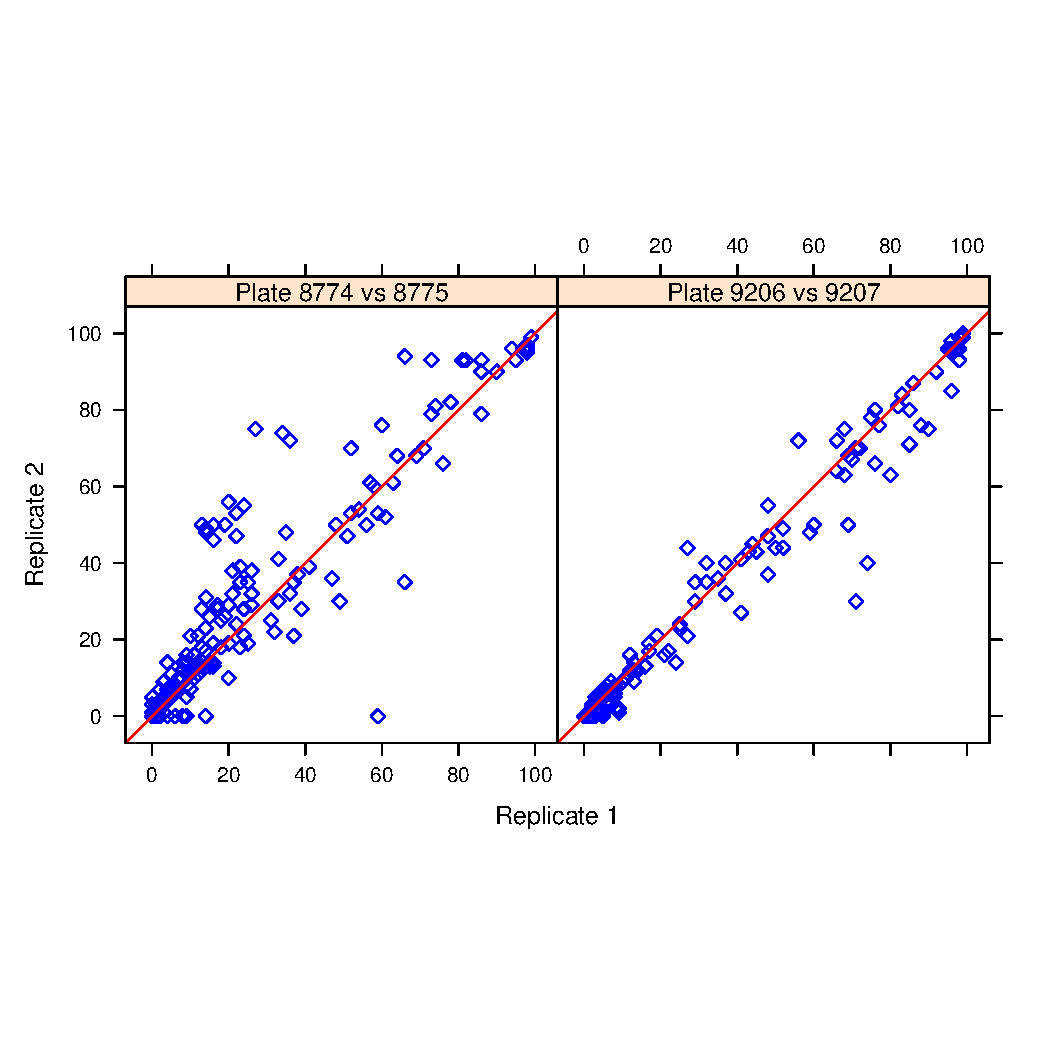
\includegraphics{replicate.pdf}
\caption{FlowJo estimates for the percentage of cells above the isotype
threshold for 189 markers on replicate plates for donor 1 and donor 2.
Estimates from markers where the center of the cell population was near the
isotype threshold, around 50\%, were more variable than samples which were
clearly positive($\ge$99\%) or negative ($\le$1\%). The correlation for
replicate plates was strong in both donors, with donor 1 at 0.92 and donor 2 at
0.98. Plate 9208 for donor 2 is not shown, since the results are very similar to
9206 and 9207.}
\label{fig:replicate}
\end{figure}

\begin{figure}
\centering
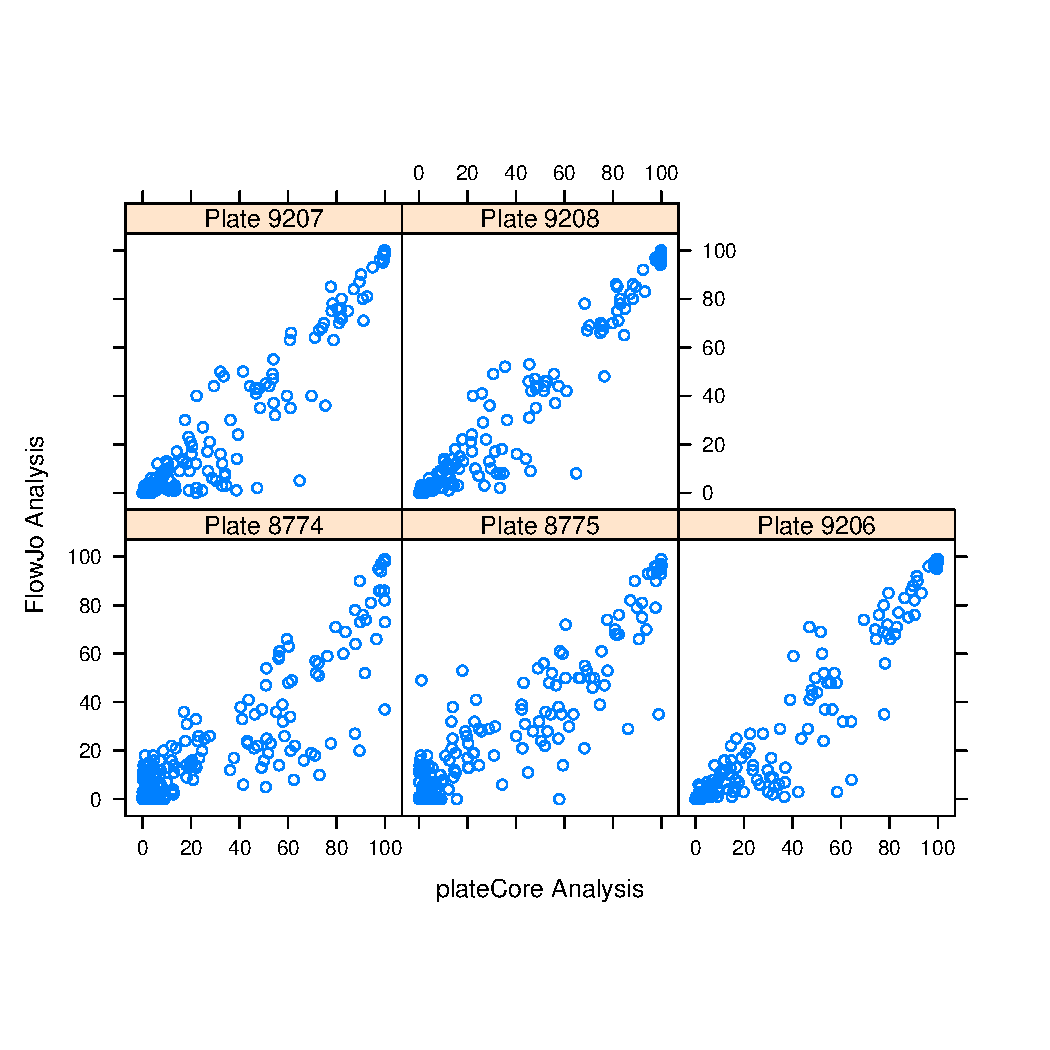
\includegraphics{fjVSr.pdf}
\caption{Plot showing the percentage of cells above the isotype threshold
from plateCore (x-axis) and FlowJo (y-axis) for each of the 189 markers on
the 5 PBMC plates. If the two methods produce similar estimates, then the
values should be near the red line (y=x). In plateCore the isotype threshold was
determined using only information from the isotype control well, while the
threshold in FlowJo may be adjusted after identifying either positively or
negatively staining test samples. Generally, these FlowJo adjustments resulted
in the isotype gate being set a higher level to exclude a negative test sample. 
The effect of increasing the isotype threshold can be seen in these plots,
where most disagreements are cases where plateCore estimates are higher than
FlowJo. Detailed plots for one marker, CD112 (red diamond), where the two
methods give different results are shown in Figure~\ref{fig:pcVSman2}.
}
\label{fig:pcVSman}
\end{figure}

\begin{figure}
\centering
\includegraphics{fjVSr3.pdf}
\caption{Density plots showing the plateCore (solid black) and FlowJo (dashed
black) isotype gates for CD112  and CD109, which shared the same isotype control
(IgG1-PE). The plateCore and FlowJo analyses gave different estimates for CD112
(see Figure~\ref{fig:pcVSman}), which was caused by the gate being moved
higher in FlowJo based on the presumed negative staining for CD109.}
\label{fig:pcVSman2}
\end{figure}

%%%%%%%%%%%%%%%%%%%%%%%%%%%%%%%%%%%%%%%%%%%%%%%%%%%%%%%%%%%%%%%%%%%%%%%%%%%%%%%
\subsection*{Gating Quality Assessment}

Since we may not always have access to output from expert cytometrists to
help determine if our automated gating is reasonable, we need an alternative
approach to assessing the quality of our isotype-based gates. The strategy we
implemented in \Rpackage{plateCore} looks at the percentage of cells above the
isotype gates versus the Median Fluorsence Intensity (MFI) ratio to see if the
gating was consistent across the experiment. The
MFI ratio is defined as the ratio of the median fluoresence signal for a marker
divided by the median signal for its isotype control. Essentially, the MFI
ratio tells us how well separated the stained test sample signal is from its
negative isotype control, and this separation is clearly related to the
percentage of cells above the isotype gate (Figure~\ref{fig:mfiRatio}).

Figure~\ref{fig:mfiRatio} shows the results of a robust logistic regression for
the percentage of positive cells on the MFI ratio for the 189 markers
from the 5 plates. The bulk of the marker values (927 out of 945) are within 2
standardized residuals from the best fit line, which is surprising since the 189
different antibodies were conjugated to different fluorophores (either Alexa
488, FITC, PE, PerCP, APC, or Alexa 647) and matched against different isotypes
(either IgG1, IgG2, IgG2a, IgG2b, IgG3, or IgM). The 18 remaining cases were
examined in detail and the isotype gates were reasonble, 


but they were
multiple populations of cells in the test well (Figure~\ref{fig:mfiRatio3}). 

\begin{figure}
\centering
\includegraphics{mfiRatioB.pdf}
\caption{Quality of the automated gating was assessed by performing a robust
logistic regression of the percentage of cells above the isotype gate on the
log transformed MFI ratio, and looking for estimates that were more than 2
standardized residuals away from the best fit line (red line). There were 18
estimates flagged in this study (red diamonds) where the value was different
than we would predict from the MFI ratio. Detailed examination of these 18
cases showed that the isotype gate settings were reasonable, but they differed
from other markers in that they had more than one population of stained cells.
Sample density plots for one of these markers, CD3, are provided in
Figure~\ref{fig:mfiRatio3}.
}
\label{fig:mfiRatio}
\end{figure}

\begin{figure}
\centering
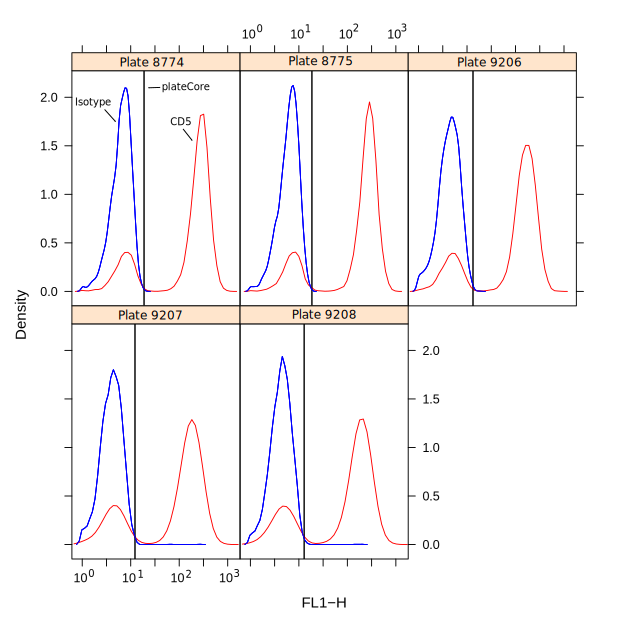
\includegraphics{mfiRatio2.pdf}
\caption{Density plot for CD3 (IgG1-Alexa 488), which was flagged for further
evaluation by our gating quality assessement (Figure~\ref{fig:mfiRatio}).
The isotype gate setings look reasonable, however the MFI ratio for CD3 was
very different from other markers that also had 75-80\% of their cells above
the isotype gate. Looking at Figure~\ref{fig:mfiRatio}, other markers with
75-80\% had MFI ratios near 5, while CD3 has an MFI ratio of 31-37. The
flagging was the result of 2 cell populations for CD3, whereas most other
markers stain a single population. }
\label{fig:mfiRatio3}
\end{figure}

%%%%%%%%%%%%%%%%%%%%%%%%%%%%%%%%%%%%%%%%%%%%%%%%%%%%%%%%%%%%%%%%%%%%%%%%%%%%%%%
\clearpage
\section*{Discussion}

We showed that the non-parametric approach to gating implemented in plateCore
produces results that are similar to those from an expert user when analyzing
PBMC lymphocyte FACS CAP data. Since this was a screening assay, the goal was to
quickly and reproducibly process a large volume of data and get an approximate
answer for each of the 189 human cell surface markers, and then perform more
in-depth analysis for markers that were of biological interest. Using
\Rpackage{plateCore}, we were able to reduce the level subjectivity in setting
isotype gates, eliminate mistakes associated with manual data annotation and
export, and automate the creation of plots and data quality reports that
summarized the experiment. Additionally, the \Rpackage{plateCore} scripts and
experimental annotation can be shared with other cytometry groups, allowing
them to reproduce our analysis.

Looking at markers where FlowJo and plateCore gave different results, such as
CD112, it is not clear that either method actually gated the cells correctly.
The gene for CD112 (PVRL2) has been shown to be expressed on a subset of B cells,
CD4 T cells, CD8 T cells, and NK cells in healthy donors using microarrays
\citep{Critchley2007}, so the plateCore results showing 65-92\% of the
lymphocytes above the isotype gate may actually represent specific staining.
Unfortunately, increasing the isotype (IGg1-PE) threshold in FlowJo to
eliminate what looks like negative, non-specific staining in CD109
(Figure~\ref{fig:pcVSman2}) also seems reasonable. More focused studies will
have to be performed to determine if the staining for CD112, and other markers
that disagreed, was positive or negative.

Another advantage of performing the analysis in plateCore is the ability to
verify that that isotype-based gate settings were consistent across the 5
PBMC plates. 


Comparing the MFI ratio to the percentage of cells above the
isotype threshold (Figure~\ref{fig:mfiRatio}) shows that there is a
relationship between the separation between a test and its control, and the
fraction of cells above the gate. While this approach does not tell us if the
gating was correct, it does help to ensure that the isotype gate for two
replicate samples was set at the same level. 

The complexity of large FCM experiments, like BD FACS CAP, highlight the 
difficulty of applying existing FCM analysis platforms to high-throughput
studies. Generating and interpreting results from this PBMC study required
extensive collaboration between flow cytometrists, bioinformaticians, and
statisticians. At various points in the analysis, each group needed to access
the raw data, annotation, and details about the experimental design. Providing
this access using stand-alone FCM platforms is expensive in terms of the price
of multiple software licenses and in time spent training statisticians and
bioinformaticians to use the programs. Fortunately the Bioconductor FCM
packages are modeled on standard data structures used for microarrays, which
should already be familiar to most quantitative individuals working on
high-throughput biological problems. We found that \Rpackage{flowCore},
\Rpackage{flowViz}, and \Rpackage{plateCore} provided an open analysis platform
that facilitated communication between the flow cytometrists generating the
data and the computational experts analyzing the data.


%Markers that are expressed on a small subset of lymphocytes, or markers that
%are dimly expressed, would not be found with this screening approach.
%(Expand - Ryan)

%While FACS CAP data
%analysis can be performed relatively quickly in FlowJo, it can be difficult to
%capture and reproduce the subjective gating decisions made by a single expert
%user. 

%In addition to subjective gating, the lack of a standard format for describing
%large FCM experiments also makes it difficult for anyone other than the
%original experimenter to replicate an analysis. (You could add something about
%MIFlowCyt here as well, as even if people had a format to follow, unless they
%put all the data in necessary to understand, just having a format isn't enough
%- Ryan) The development of mechanism to bundle experimental metadata
%descriptions with FCS data files should make it easier to access metadata in
%future FCM studies, but currently this information is typically provided either
%as spreadsheet or a pictorial layout of a 96 well plate. Since the creation of
%\Robject{flowPlate} requires users to make a standard sample annotation file,
%plate layouts from \Rpackage{plateCore} can then be easily shared along with
%the raw FCS2.0/3.0 files. The standard format for \Rpackage{plateCore} sample
%annotations provides a convenient way to manage the plate metadata associated
%with complex FC-HCS experiments.

%%%%%%%%%%%%%%%%%%%%%%%%%%%%%%%%%%%%%%%%%%%%%%%%%%%%%%%%%%%%%%%%%%%%%%%%%%%%%%%
\clearpage
\bibliographystyle{plain}
\bibliography{outline} 

\end{document}
